% https://tex.stackexchange.com/questions/58249/how-to-shade-mindmap-concepts?rq=1
\documentclass[a4paper,11pt]{standalone}
\usepackage{tikz}
\usetikzlibrary{mindmap}

\tikzset{level 1 concept/.append style={font=\sf, sibling angle=90,level distance = 25mm}}
\tikzset{level 2 concept/.append style={font=\sf, sibling angle=45,level distance = 16mm}}
\tikzset{level 3 concept/.append style={font=\sf, sibling angle=45,level distance = 17mm}}
\tikzset{every node/.append style={scale=0.6}}

\begin{document}

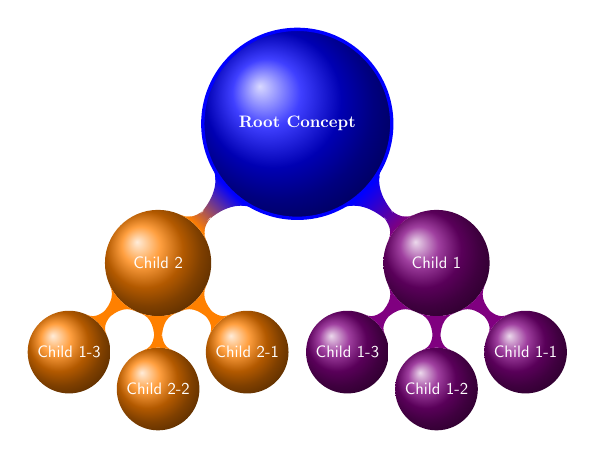
\begin{tikzpicture}
    [
        mindmap, 
        concept color=blue, 
        font=\sf\bf, 
        text=white
    ]
    \node[concept,ball color=blue]{Root Concept}[clockwise from=315]
    child [concept color=violet] {node[circle,ball color=violet] (c1){Child 1}                                
        child  {node [circle,ball color=violet](c11){Child 1-1}}
        child  {node [circle,ball color=violet](c12){Child 1-2}}
        child  {node [circle,ball color=violet](c13){Child 1-3}}                                                   
    }
    child [concept color=orange]{node [circle,ball color=orange](c2){Child 2}
        child {node [circle,ball color=orange](c21){Child 2-1}}
        child {node [circle,ball color=orange](c22){Child 2-2}}
        child {node [circle,ball color=orange](c22){Child 1-3}}
    };
\end{tikzpicture}
\end{document}